\documentclass{article}
\usepackage{amsmath}
\usepackage{amssymb}
\usepackage{graphicx}
\usepackage{hyperref}
\usepackage[version=4]{mhchem}

\title{Example 2}
\date{}

\begin{document}
\maketitle

As shown in the figure, three circles are externally tangent. \(P C A\) and \(P D B\) are common tangents. \(D\) and \(E\) are the tangent points and are also the midpoints of \(P B\) and \(P D\) respectively. Find the area of the largest circle if \(P B=12\).\\
(A) \(14 \pi\)\\
(B) \(18 \pi\)\\
(C) \(25 \pi\)\\
(D) \(24 \pi\)\\
(E) \(14 \pi\)\\
\centering
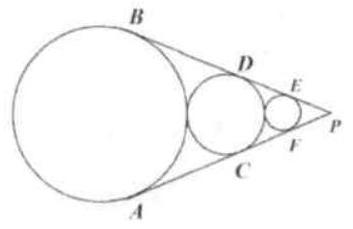
\includegraphics[width=\textwidth]{images/problem_image_1.jpg}

Solution: (B).\\
Connect \(P O^{\prime \prime}, B O^{\prime \prime}, D O^{\prime}\), and \(O E . P E=D E=3\).\\
\(B D=6 . O^{\prime \prime} B \perp P B, O^{\prime} D \perp P B, O E \perp P B\).\\
\(O E=r . O D^{\prime}=2 r . O^{\prime \prime} B=4 r . O^{\prime \prime} O^{\prime}=O^{\prime} P=6 r\).\\
By the Pythagorean Theorem in right triangle \(P O^{\prime \prime} B\),\\
\centering
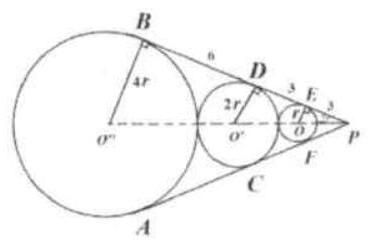
\includegraphics[width=\textwidth]{images/reasoning_image_1.jpg}\\
\(P O^{\prime \prime 2}=P B^{2}+O^{\prime \prime} B^{2} \Rightarrow 144+16 r^{2}=144 r^{2} \quad \Rightarrow(4 r)^{2}=18\).


The area of the largest circle is \(18 \pi\).\\

\end{document}
